\subsection{The MOUS dataset}

Next, we apply our method to brain imaging data, on the ``Mother Of all Unification
Studies'' (MOUS) dataset \cite{schoffelen2019204}. The dataset consists of
anonymized multimodal neuroimaging data that has been acquired from 204 healthy
human subjects, which participated in either a auditory or a visual version of a
language experiment. In this work, we use the subset corresponding to the visual
variant recorded using magneto-encephalography (MEG).

Subjects were presented a set of 120 sentences in Dutch, and scrambled lists
of the same words for a controlled experiment. Each word was presented on a
screen for no less than 300 ms and no more than 1400ms, 351 ms on average.
Successive words were separated by an empty screen for 300ms, and successive
sentences were separated by an empty screen for a few (3-4) seconds.

The data contains the timestamp for each word presentation, allowing to align
time series to stimuli onsets for all words.

As a result, we obtain, for each of the 301 channels (273 magnetometers on the
subject and 28 compensation channels measuring the room) and each word
presented, a time series of 67 real-values spanning $\left[-100ms, 1000ms\right]$ relative to
the stimulus onset. Each of the 102 subjects (we used data from 93 subjects) was
presented approximately 2700 words during the experiment.

We show, in Figure \ref{fig:megavg}, the average response across words of the 
magnetometers for the first subject. Time $t=0$ corresponds to the stimulus onset.

\begin{figure}
  \centering
  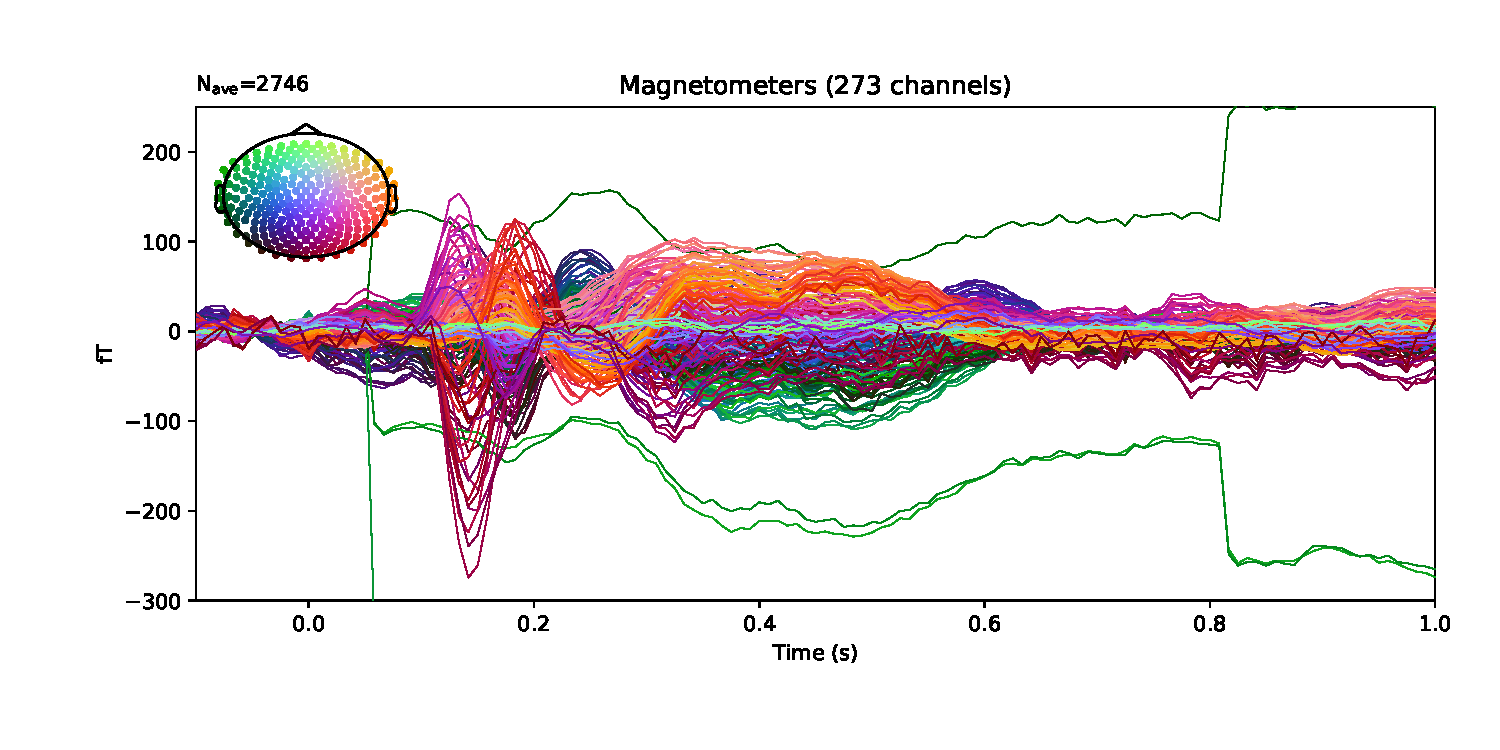
\includegraphics[width=\textwidth, trim=1.5cm 1cm 0.5cm 0cm, clip=True]{figure_meg.pdf}
  \caption{Average magnetosensor response across words for one subject.}
  \label{fig:megavg}
\end{figure}

\subsection{Application of the method}

Using this dataset, we study which features of input words can elicit a strong
MEG response in the brain.  We add to each word (i) visual features: word length
(1 dim.), letter count (26 dim.), and (ii) lexical features : word frequency (1
dim.) part-of-speech tag (one of ADJ, ADP, ADV, CONJ, DET, NOUN, NUM, PRON,
PROPN, VERB; 10 dim.). Sentence-level word features are left for future study.

This procedure yields an $\left(n \times 38\right)$-dimensional input matrix $X$,
where $n$ is the number of words for the subject. Each feature in $X$ is centered and
scaled for zero mean and unit variance.

Then, we apply the BFR method independently on each of the 67 time slices of the
MEG recordings. Each slice $Y_t$ is a $n \times 301$ matrix, also centered and
scaled. We obtain a vector of 38 coefficients per slice.

We show these coefficients as a function of time in the stacked plots, in Figure
\ref{fig:megresult}.

\begin{figure}
  \centering
  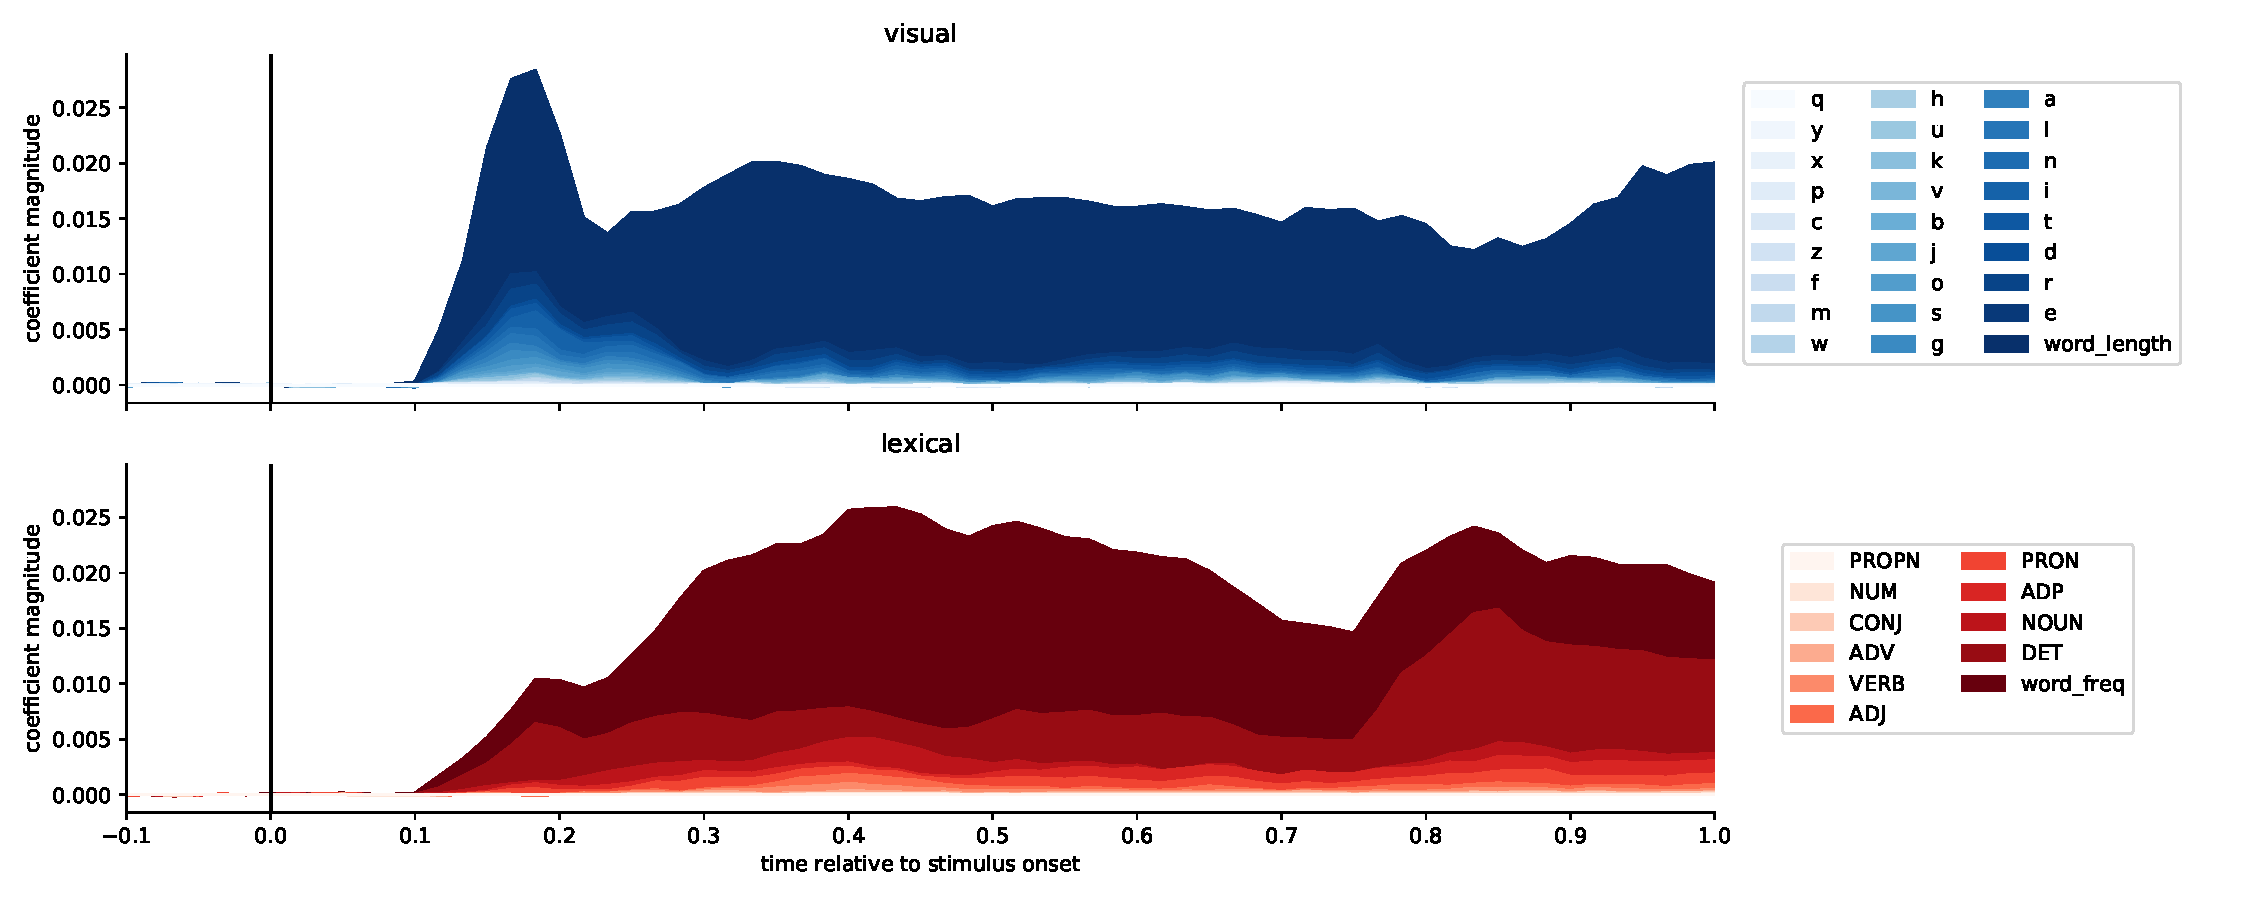
\includegraphics[width=\textwidth, trim=1.5cm 1cm 0.5cm 0cm,
clip=True]{meg_result.pdf}
  \caption{Average magnetosensor response across words for one subject.}
  \label{fig:megresult}
\end{figure}


\subsection{Discussion of the results.}

\subsubsection{Overview}


